%\documentclass[ignorenonframetext,xcolor=svgnames,hyperref={xetex,colorlinks,linkcolor=blue},compress]{beamer}

\usepackage{pgfpages}

\usepackage[backend=biber,style=alphabetic,url=false]{biblatex}
\addbibresource{os.bib}

\usepackage{latexsym,pifont,units,amsmath,amsfonts,amssymb,marvosym}
\usepackage{xltxtra} %fontspec,xunicode are loaded here.
\defaultfontfeatures{Mapping=tex-text}
\setmainfont{DejaVu Serif}
\setsansfont{DejaVu Sans}

\usepackage{xeCJK}
\setCJKmainfont[BoldFont={WenQuanYi Zen Hei}, ItalicFont={WenQuanYi Zen Hei}]{SimSun}
\setCJKfamilyfont{hei}{WenQuanYi Zen Hei}
\setCJKfamilyfont{song}{SimSun}


% \usepackage{graphicx} % beamer loads graphicx already.
\graphicspath{{./figs/}{../figs/}{./}{../}} %note that the trailing “/” is required

\usepackage{tikz}
\usetikzlibrary{arrows,decorations.pathmorphing,backgrounds,positioning,fit}

\usepackage{multicol,varwidth}

\newcommand{\cfbox}[2]{%
  \colorlet{currentcolor}{.}%
  {\color{#1}\fbox{\color{currentcolor}#2}}%
}

\newcommand{\code}[1]{\texttt{\textcolor{violet}{#1}}}

\mode<beamer>{
  \usetheme{default}
  \usecolortheme{sidebartab}
  \usefonttheme{serif}
  \setbeamertemplate{footline}[frame number]
  \setbeamertemplate{navigation symbols}{}
  \usenavigationsymbolstemplate{}
  \setbeamertemplate{blocks}[rounded][shadow=true]
  \setbeamercolor{structure}{fg=Green}
  \setbeamercolor{block title}{fg=Green}
}

\begin{document}

\mode<article>{
  \title{Course Introduction}
  \author{Wang Xiaolin\\wx672ster@gmail.com}
  \maketitle
%  \tableofcontents
%  \clearpage
}

\begin{frame}<beamer>
  \title{Course Introduction}
  \author{Wang Xiaolin}
  \titlepage
  \vfill
  \tiny{
    \ding{41} wx672ster+os@gmail.com
    % \ding{37}
  }
\end{frame}


\begin{frame}{Theory vs. Practice}
  \begin{center}
    \textcolor{blue}{\emph{``which came first, the chicken or the egg?''}}
  \end{center}
  \begin{description}
  \item[OS Concepts:] theories about how OS works
  \item[Linux System Analysis:] \ \\
    \begin{itemize}
    \item implementation
    \item engineering
    \item practice
    \item OS concepts + Programming(c, assembly)
    \end{itemize}
  \end{description}
\end{frame}

\begin{frame}{OS Fundamentals}
  \begin{refsection}
    \nocite{tanenbaum2008modern, silberschatz11essentials, zouhengming09}
    \printbibliography[heading=none]
  \end{refsection}
\end{frame}

\begin{frame}{Linux Kernel}
  \begin{refsection}
    \nocite{corbet05:_linux_devic_driver, bovet2005understanding, mauerer2008professional,
      love2010linux, rodriguez2005linux}
    \printbibliography[heading=none]
  \end{refsection}
\end{frame}

\begin{frame}{Assembly and C Programming}
  \begin{refsection}
    \nocite{bartlett2009programming, carter06:_pc_assem_languag, x86assemblymanual,
      wikibooks-gas, gcc-inline-asm, x86-inline-asm-linux, gcc-gen-asm}
    \printbibliography[heading=none]
  \end{refsection}
\end{frame}

\begin{frame}{Lab References}
  \begin{refsection}
    \nocite{kroah-hartman07:_linux_kernel_nutsh, yuyuan2009orange}
    \printbibliography[heading=none]
  \end{refsection}
\end{frame}

\begin{frame}{Web Resources}
  \begin{thebibliography}{}
  \bibitem{} \href{http://cs3.swfu.edu.cn/moodle/course/view.php?id=2737}{Course web site}
  \bibitem{} \href{http://cs3.swfu.edu.cn/phpbb/viewforum.php?f=10}{Course discussion board}
  \bibitem{} \href{http://wikipedia.org}{Wikipedia}
  \bibitem{} \href{http://wiki.osdev.org/}{OSDev}
  \end{thebibliography}
\end{frame}

\begin{frame}{Grading}
  \begin{exampleblock}{No exam!}
    \begin{equation*}
      \text{Final mark} =
      \begin{cases}
        1/3& \text{assignments}\\
        1/3& \text{class participation}\\
        1/3& \text{project}
      \end{cases}
    \end{equation*}
  \end{exampleblock}
    \begin{description}
  \item[Assignments:] Lab works
  \item[Class participation:]\ 
    \begin{itemize}
    \item Class attendance
    \item Using Linux to do your daily work
    \item Asking questions
    \item BBS posting
    \item ...
    \end{itemize}
  \item[Project:] \ 
    \begin{itemize}
    \item Follow \href{http://cs2.swfu.edu.cn/pub/resources/Books/OS/OrangeS/}{Orange'S} to write a simple OS
    \item Write something meaningful
    \end{itemize}
  \end{description}
\end{frame}

\begin{frame}{Linux Kernel Development}{--- Google Tech Talks}
  \begin{thebibliography}{}
  \bibitem[]{} \href{http://www.youtube.com/watch?v=L2SED6sewRw}{Google Tech Talks ---
      Greg Kroah Hartman on the Linux Kernel}
  \end{thebibliography}
\end{frame}

\begin{frame}{Lines of Code}
  \begin{exampleblock}{Per day 2007 - 2008}
    \begin{itemize}
    \item 4,300 lines added
    \item 1,800 lines removed
    \item 1,500 lines modified
    \end{itemize}
  \end{exampleblock}
  % \begin{center}
  %   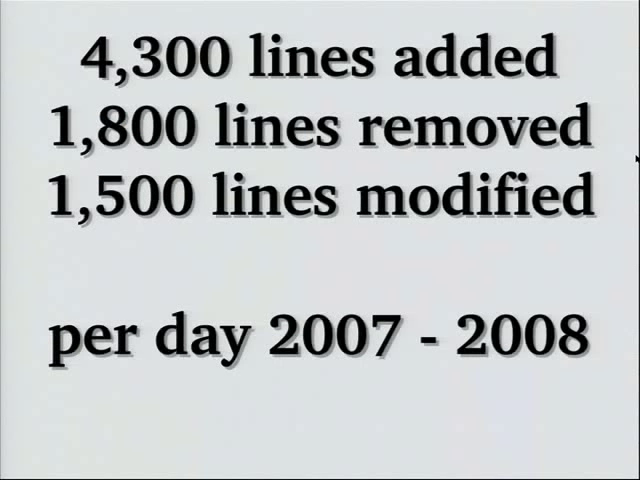
\includegraphics[width=\textwidth]{shot0001}
  % \end{center}
\end{frame}

\begin{frame}
  \begin{center}
    \mode<beamer>{
      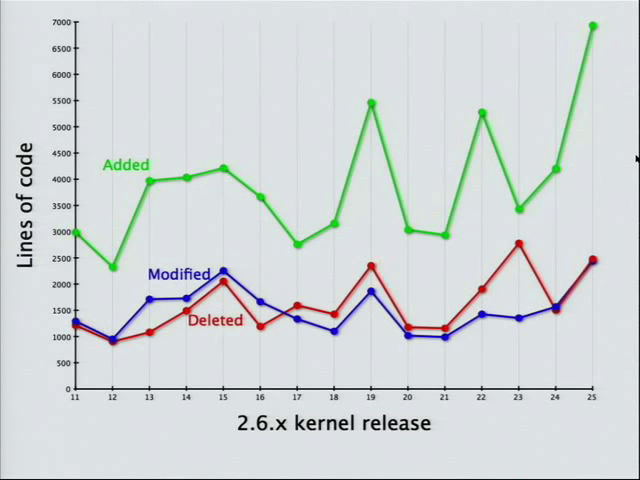
\includegraphics[width=\textwidth]{shot0002}
    }
    \mode<article>{
      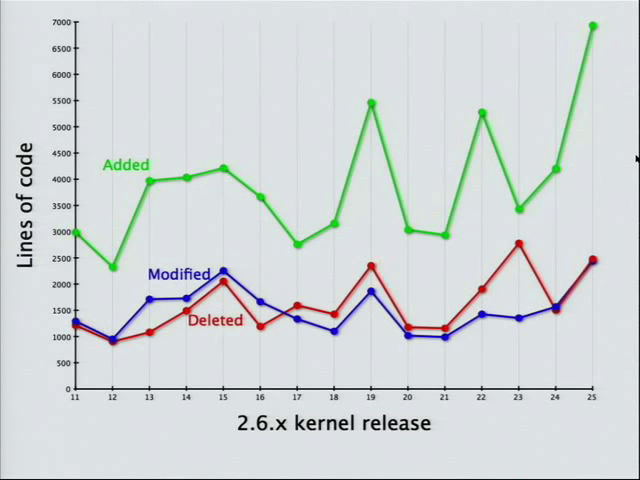
\includegraphics[width=.6\textwidth]{shot0002}
    }
  \end{center}
\end{frame}

\begin{frame}{3.69 Changes Per Hour}
  \begin{center}
    \mode<beamer>{
      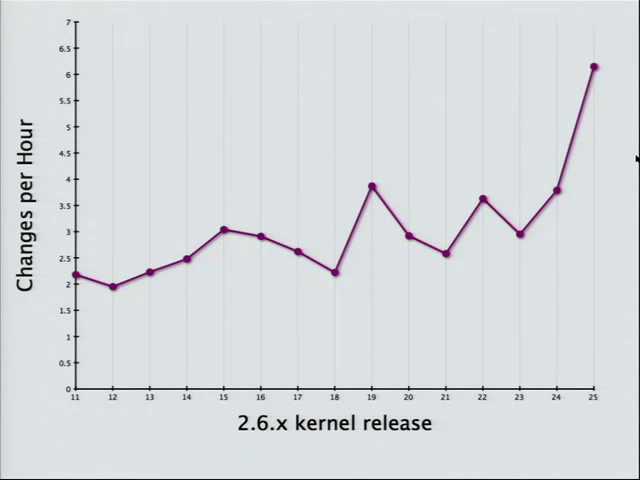
\includegraphics[width=\textwidth]{shot0004}
    }
    \mode<article>{
      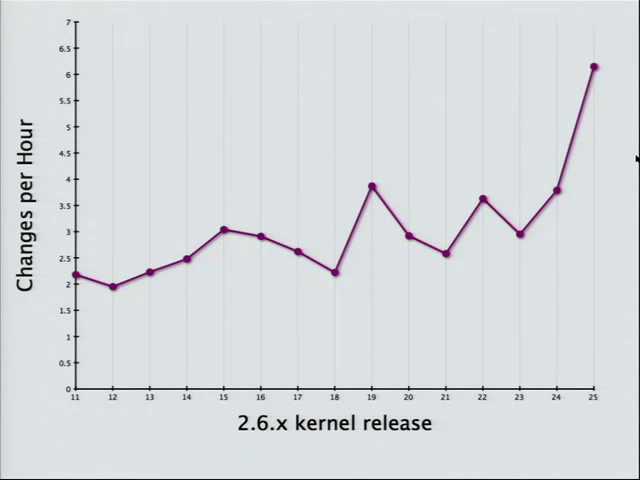
\includegraphics[width=.6\textwidth]{shot0004}
    }
  \end{center}
\end{frame}

% \begin{frame}
  
%   % \begin{center}
%   %   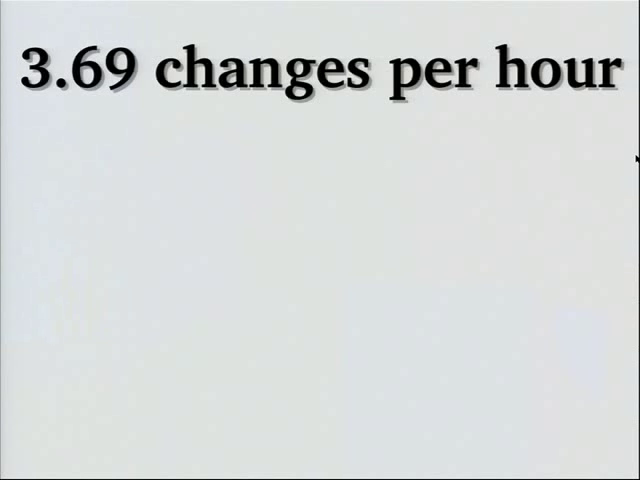
\includegraphics[width=\textwidth]{shot0005}
%   % \end{center}
% \end{frame}

\begin{frame}
  \begin{center}
    \mode<beamer>{
      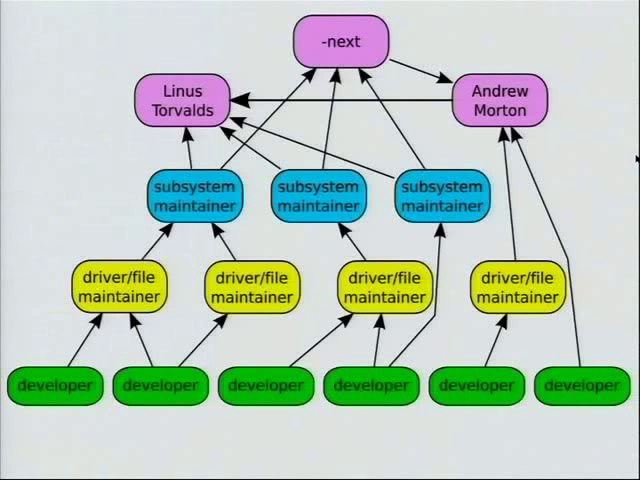
\includegraphics[width=\textwidth]{shot0003}
    }
    \mode<article>{
      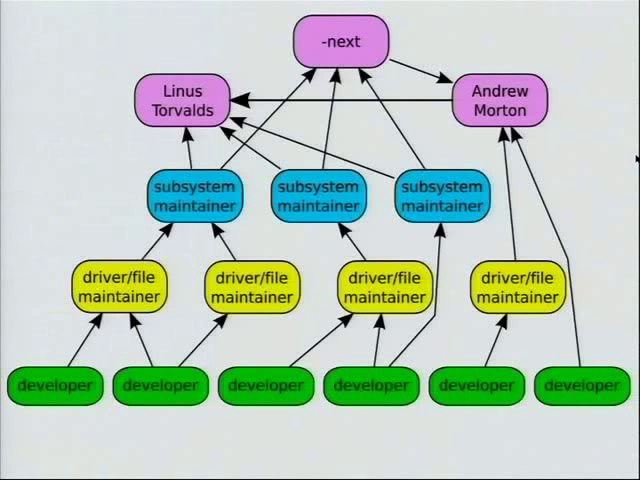
\includegraphics[width=.6\textwidth]{shot0003}
    }
  \end{center}
\end{frame}

\begin{frame}
  \begin{center}
    \mode<beamer>{
      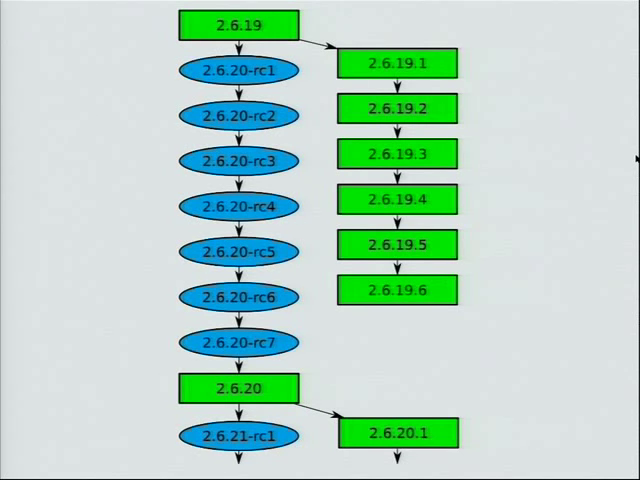
\includegraphics[width=\textwidth]{shot0006}
    }
    \mode<article>{
      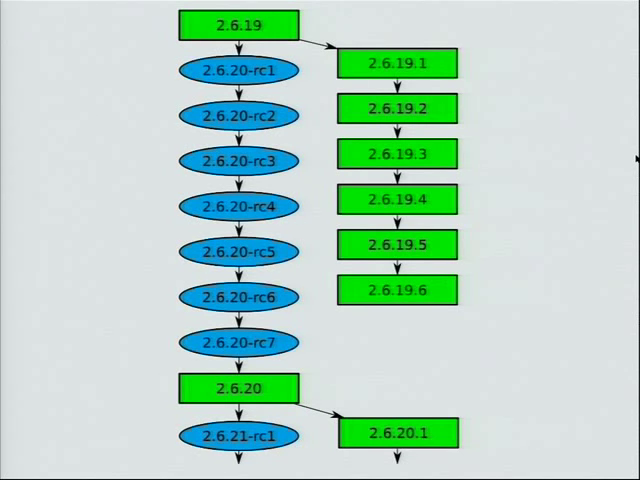
\includegraphics[width=.6\textwidth]{shot0006}
    }
  \end{center}
\end{frame}

\begin{frame}
  \begin{itemize}
  \item New releases every $2\frac{3}{4}$ months
  \item 9.2 million lines as of the 2.6.25 release
  \item 2399 developers (2.6.20 $\sim$ 2.6.25)
  \end{itemize}
  % \begin{center}
  %   
\includegraphics[width=\textwidth]{shot0007}
  % \end{center}
\end{frame}

% \begin{frame}
%   \begin{center}
%     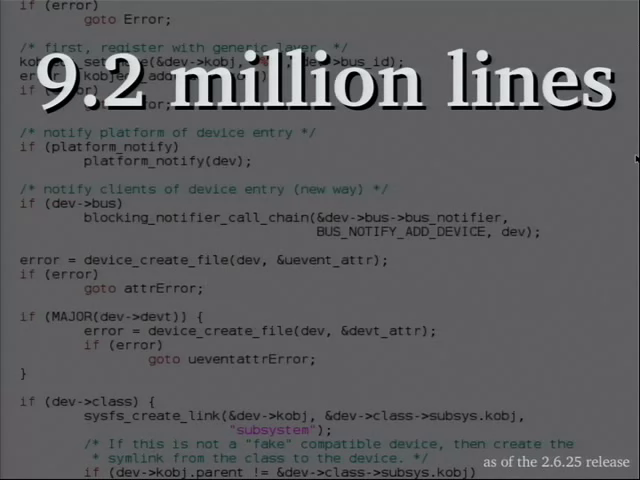
\includegraphics[width=\textwidth]{shot0008}
%   \end{center}
% \end{frame}

% \begin{frame}
%   \begin{center}
%     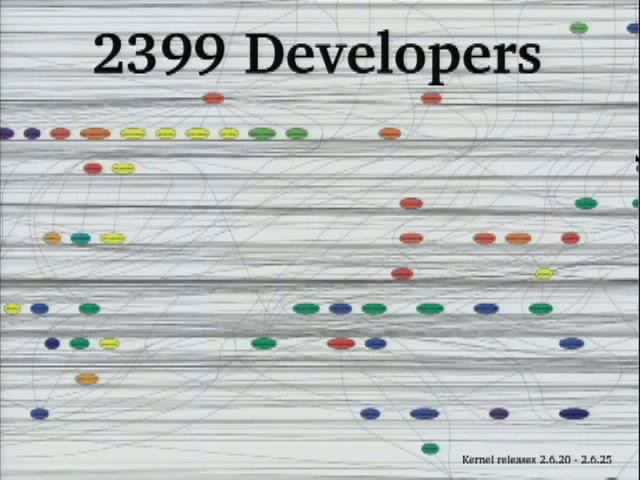
\includegraphics[width=\textwidth]{shot0009}
%   \end{center}
% \end{frame}

\begin{frame}%{top developers}
  \begin{center}
    \mode<beamer>{
      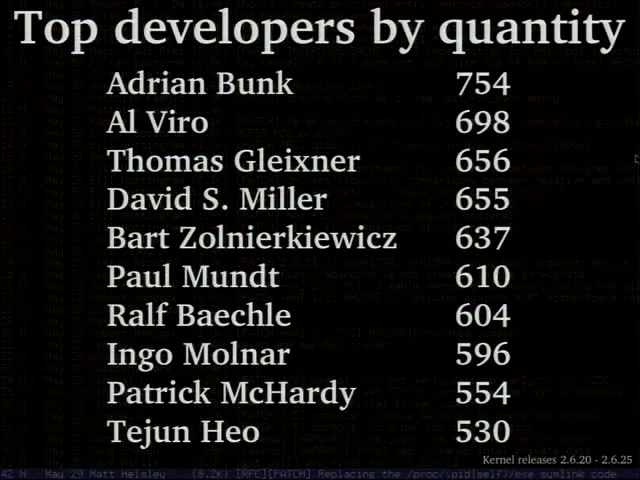
\includegraphics[width=\textwidth]{shot0010}
    }
    \mode<article>{
      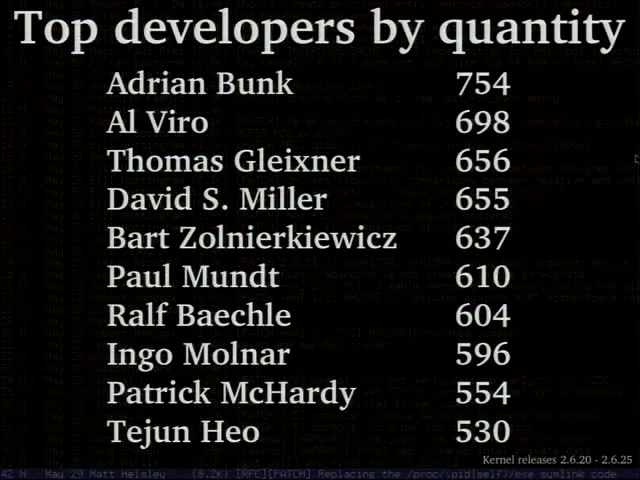
\includegraphics[width=.6\textwidth]{shot0010}
    }
  \end{center}
\end{frame}

\begin{frame}%{top signed-off-by}
  \begin{center}
    \mode<beamer>{
      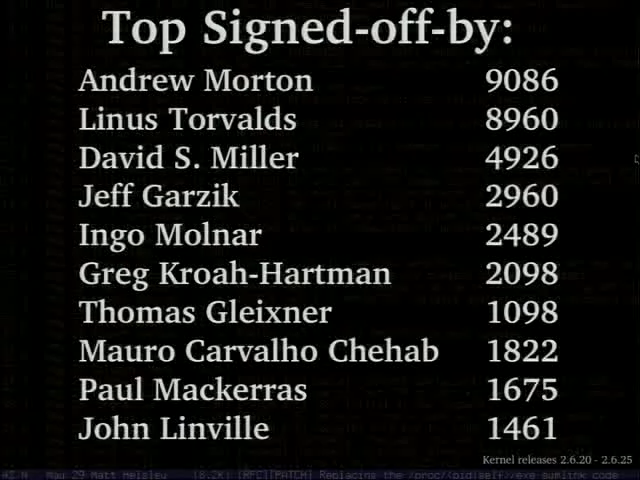
\includegraphics[width=\textwidth]{shot0011}
    }
    \mode<article>{
      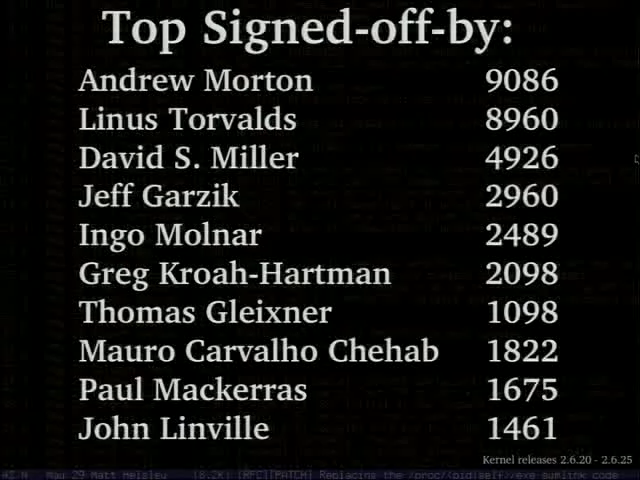
\includegraphics[width=.6\textwidth]{shot0011}
    }
  \end{center}
\end{frame}

\begin{frame}%{Who is funding this work?1}
  \begin{center}
    \mode<beamer>{
      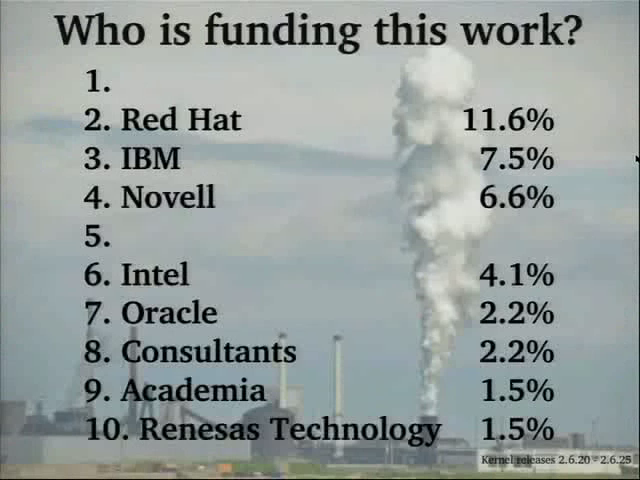
\includegraphics[width=\textwidth]{shot0012}
    }
    \mode<article>{
      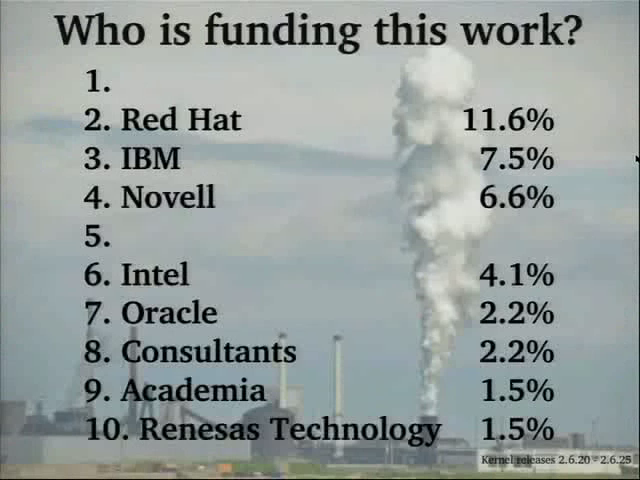
\includegraphics[width=.6\textwidth]{shot0012}
    }
  \end{center}
\end{frame}

\begin{frame}%{Who is funding this work?2}
  \begin{center}
    \mode<beamer>{
      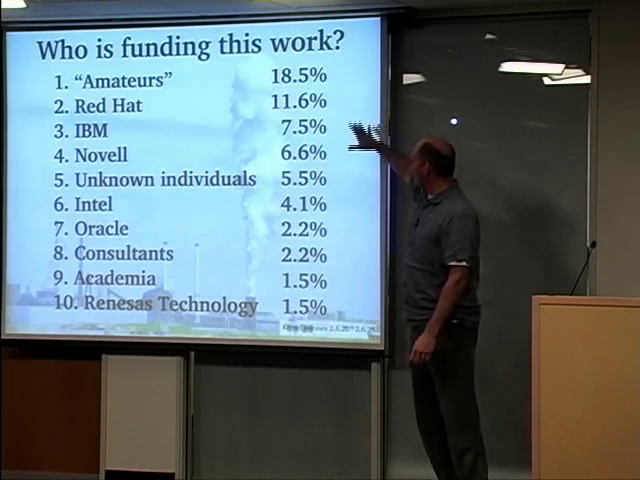
\includegraphics[width=\textwidth]{shot0013}
    }
    \mode<article>{
      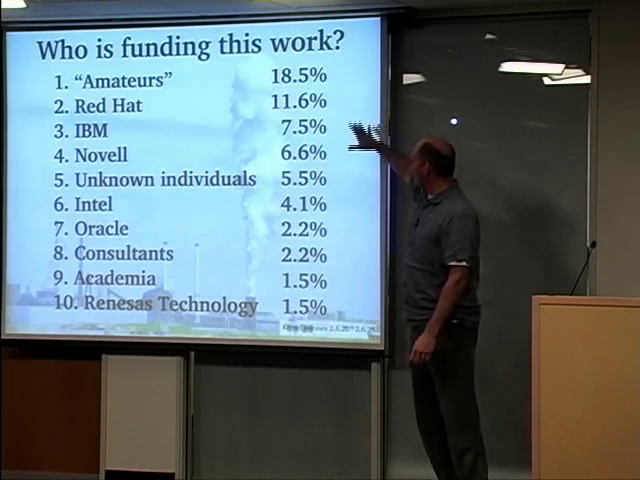
\includegraphics[width=.6\textwidth]{shot0013}
    }
  \end{center}
\end{frame}

\begin{frame}%{Who is funding this work?3}
  \begin{center}
    \mode<beamer>{
      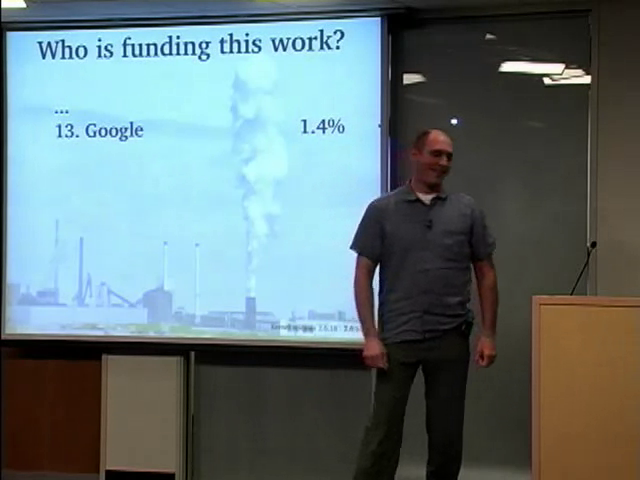
\includegraphics[width=\textwidth]{shot0015}
    }
    \mode<article>{
      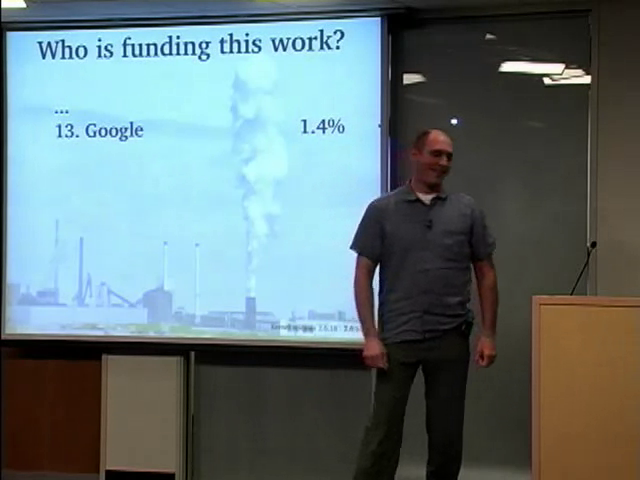
\includegraphics[width=.6\textwidth]{shot0015}
    }
  \end{center}
\end{frame}

\begin{frame}%{Who is funding this work?4}
  \begin{center}
    \mode<beamer>{
      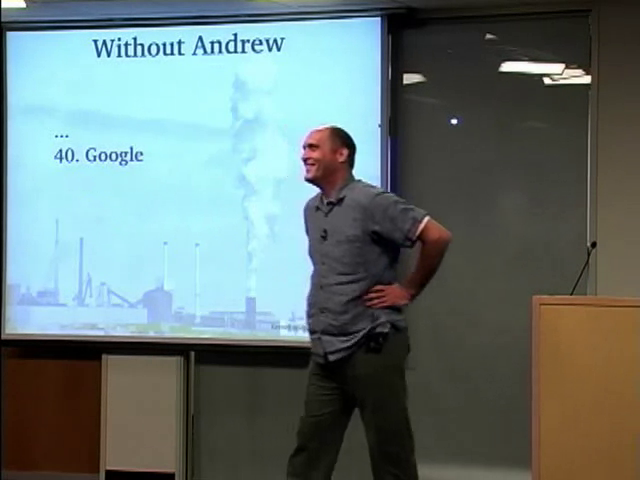
\includegraphics[width=\textwidth]{shot0014}
    }
    \mode<article>{
      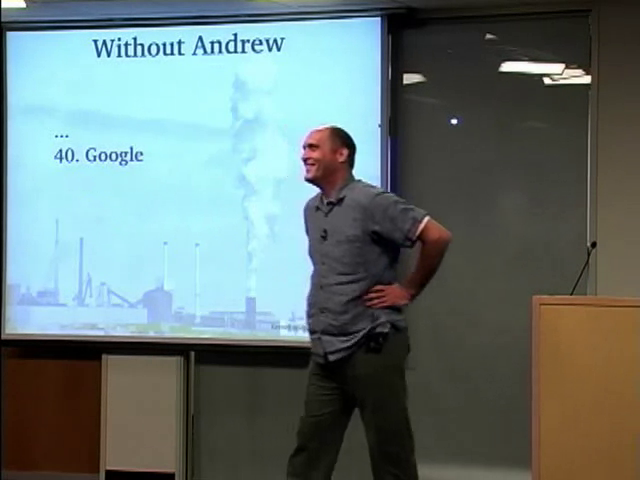
\includegraphics[width=.6\textwidth]{shot0014}
    }
  \end{center}
\end{frame}

\begin{frame}
  27 Google employees contributed to the kernel in 2007-2008
  % \begin{center}
  %   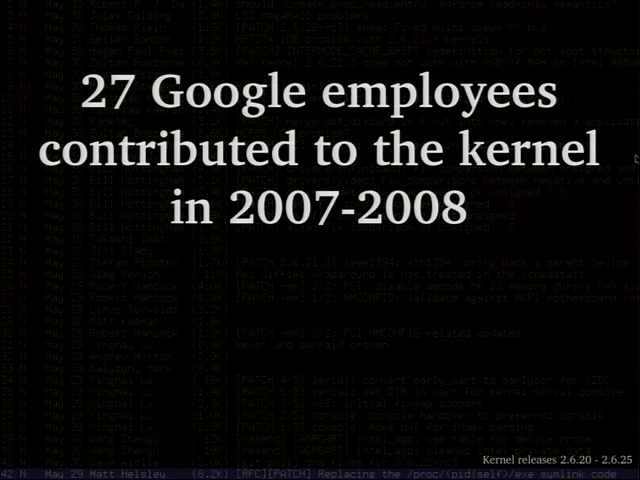
\includegraphics[width=\textwidth]{shot0016}
  % \end{center}
\end{frame}

\begin{frame}%{Google employee contributions}
  \begin{center}
    \mode<beamer>{
      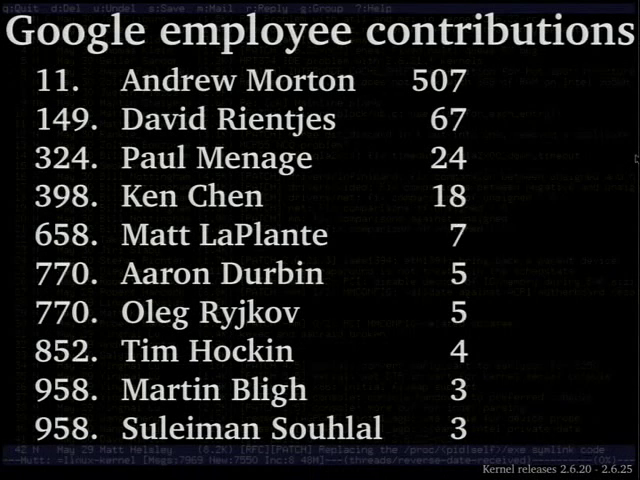
\includegraphics[width=\textwidth]{shot0017}
    }
    \mode<article>{
      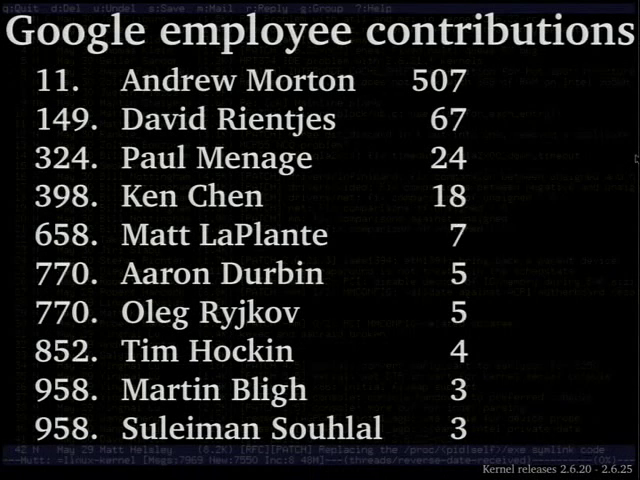
\includegraphics[width=.6\textwidth]{shot0017}
    }
  \end{center}
\end{frame}

\begin{frame}%{Google employee contributions 2}
  \begin{center}
    \mode<beamer>{
      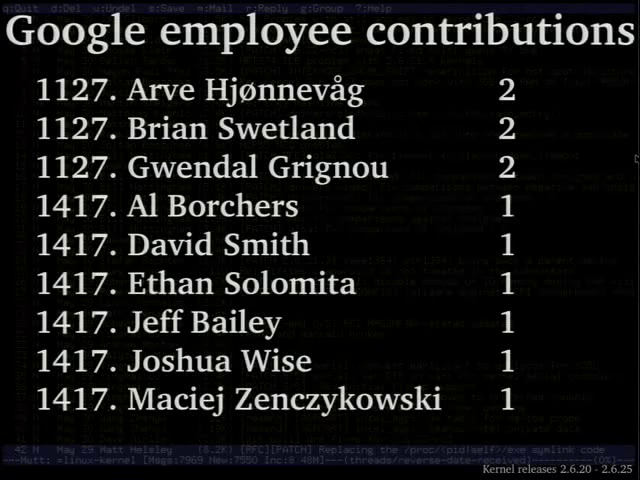
\includegraphics[width=\textwidth]{shot0018}
    }
    \mode<article>{
      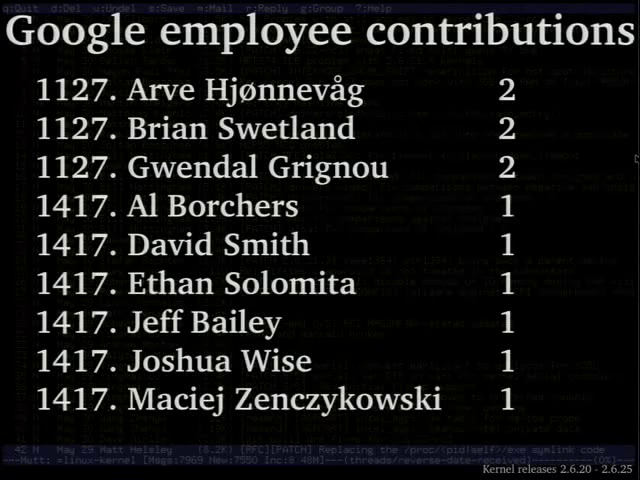
\includegraphics[width=.6\textwidth]{shot0018}
    }
  \end{center}
\end{frame}

\begin{frame}%{Google employee contributions 3}
  \begin{center}
    \mode<beamer>{
      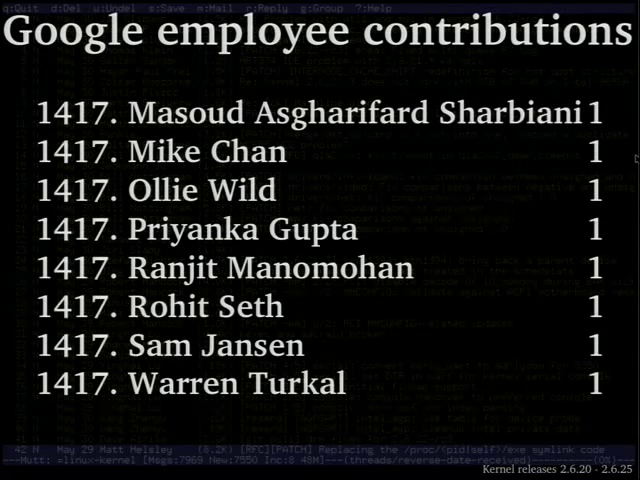
\includegraphics[width=\textwidth]{shot0020}
    } \mode<article>{
      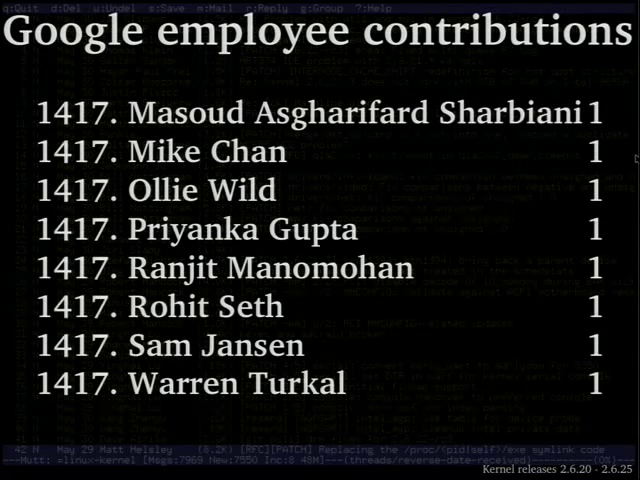
\includegraphics[width=.6\textwidth]{shot0020}
    }
  \end{center}
\end{frame}

\begin{frame}%{New stuff in 2.6.26}
  \begin{center}
    \mode<beamer>{
      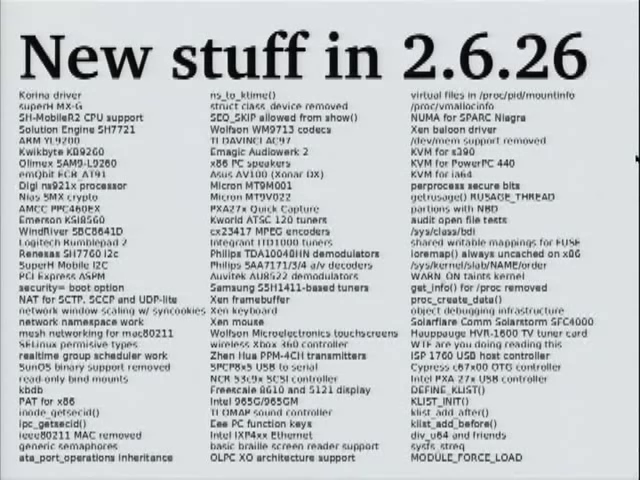
\includegraphics[width=\textwidth]{shot0019}
    }
    \mode<article>{
      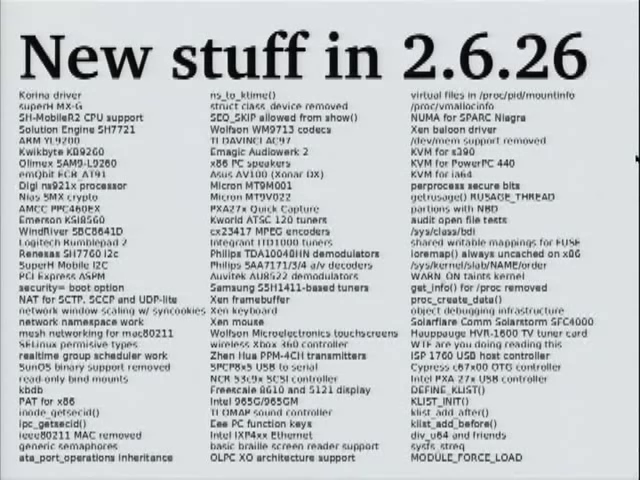
\includegraphics[width=.6\textwidth]{shot0019}
    }
  \end{center}
\end{frame}

\end{document}
